\subsection{シミュレータ}
最適化の方法として, 複数のパラメータからモデルと実行環境に即したパラメータを選択するという手法を選択したが,
そのためには複数のパラメータでシミュレーションを行いその結果を集約するプログラムが必要となる.\\
本研究ではこのパラメータ選択を容易かつ高速に行うため,
\begin{itemize}
\item MODファイルからパラメータとなりうる情報を自動で抽出し,パラメータの候補を生成する.
\item キューイングシステムに対して,複数のジョブを並行して投げ結果を非同期的に集約できる.
\item 実行結果を最適化前のデフォルトの結果と比較し,最適化を通して実行結果に変化がないかを確認する.
\item json形式で, 実行するファイルや各パラメータの範囲(プロセス数は1から10など)といったシミュレーションに関する情報を指定することができる.
\end{itemize}
という機能を持ったシミュレータの開発を行った.\\

\begin{figure}[h!]
% h:here, t:top, b:bottom, p:page
 \begin{center}
%    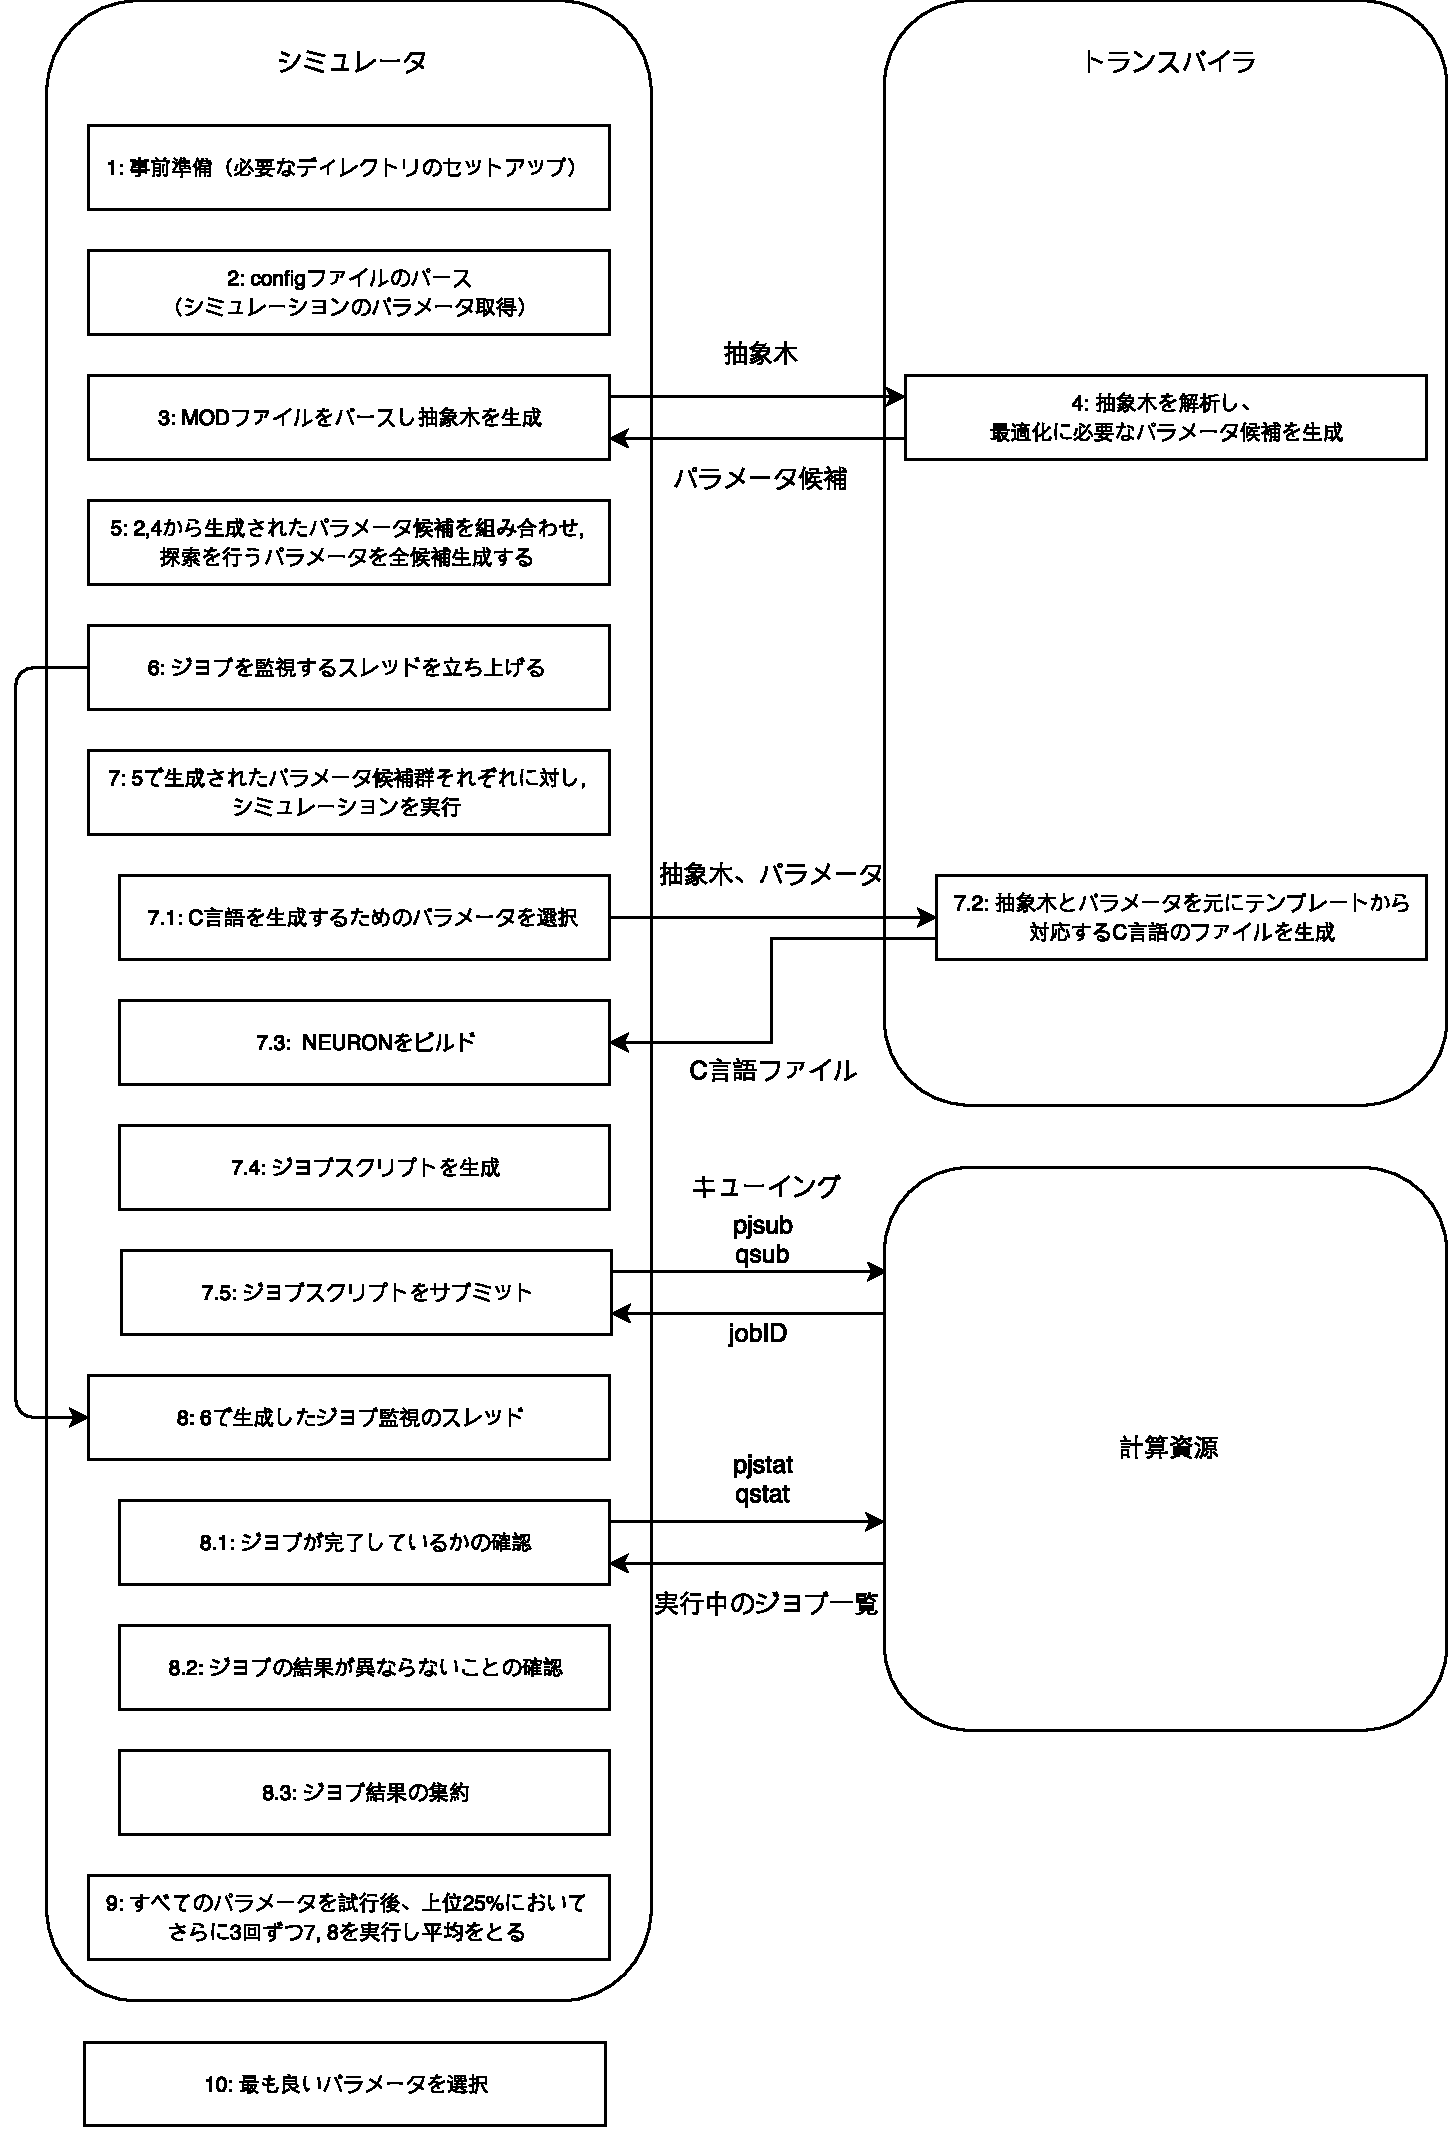
\includegraphics[width=18.0cm]{./images/Genie.pdf}
    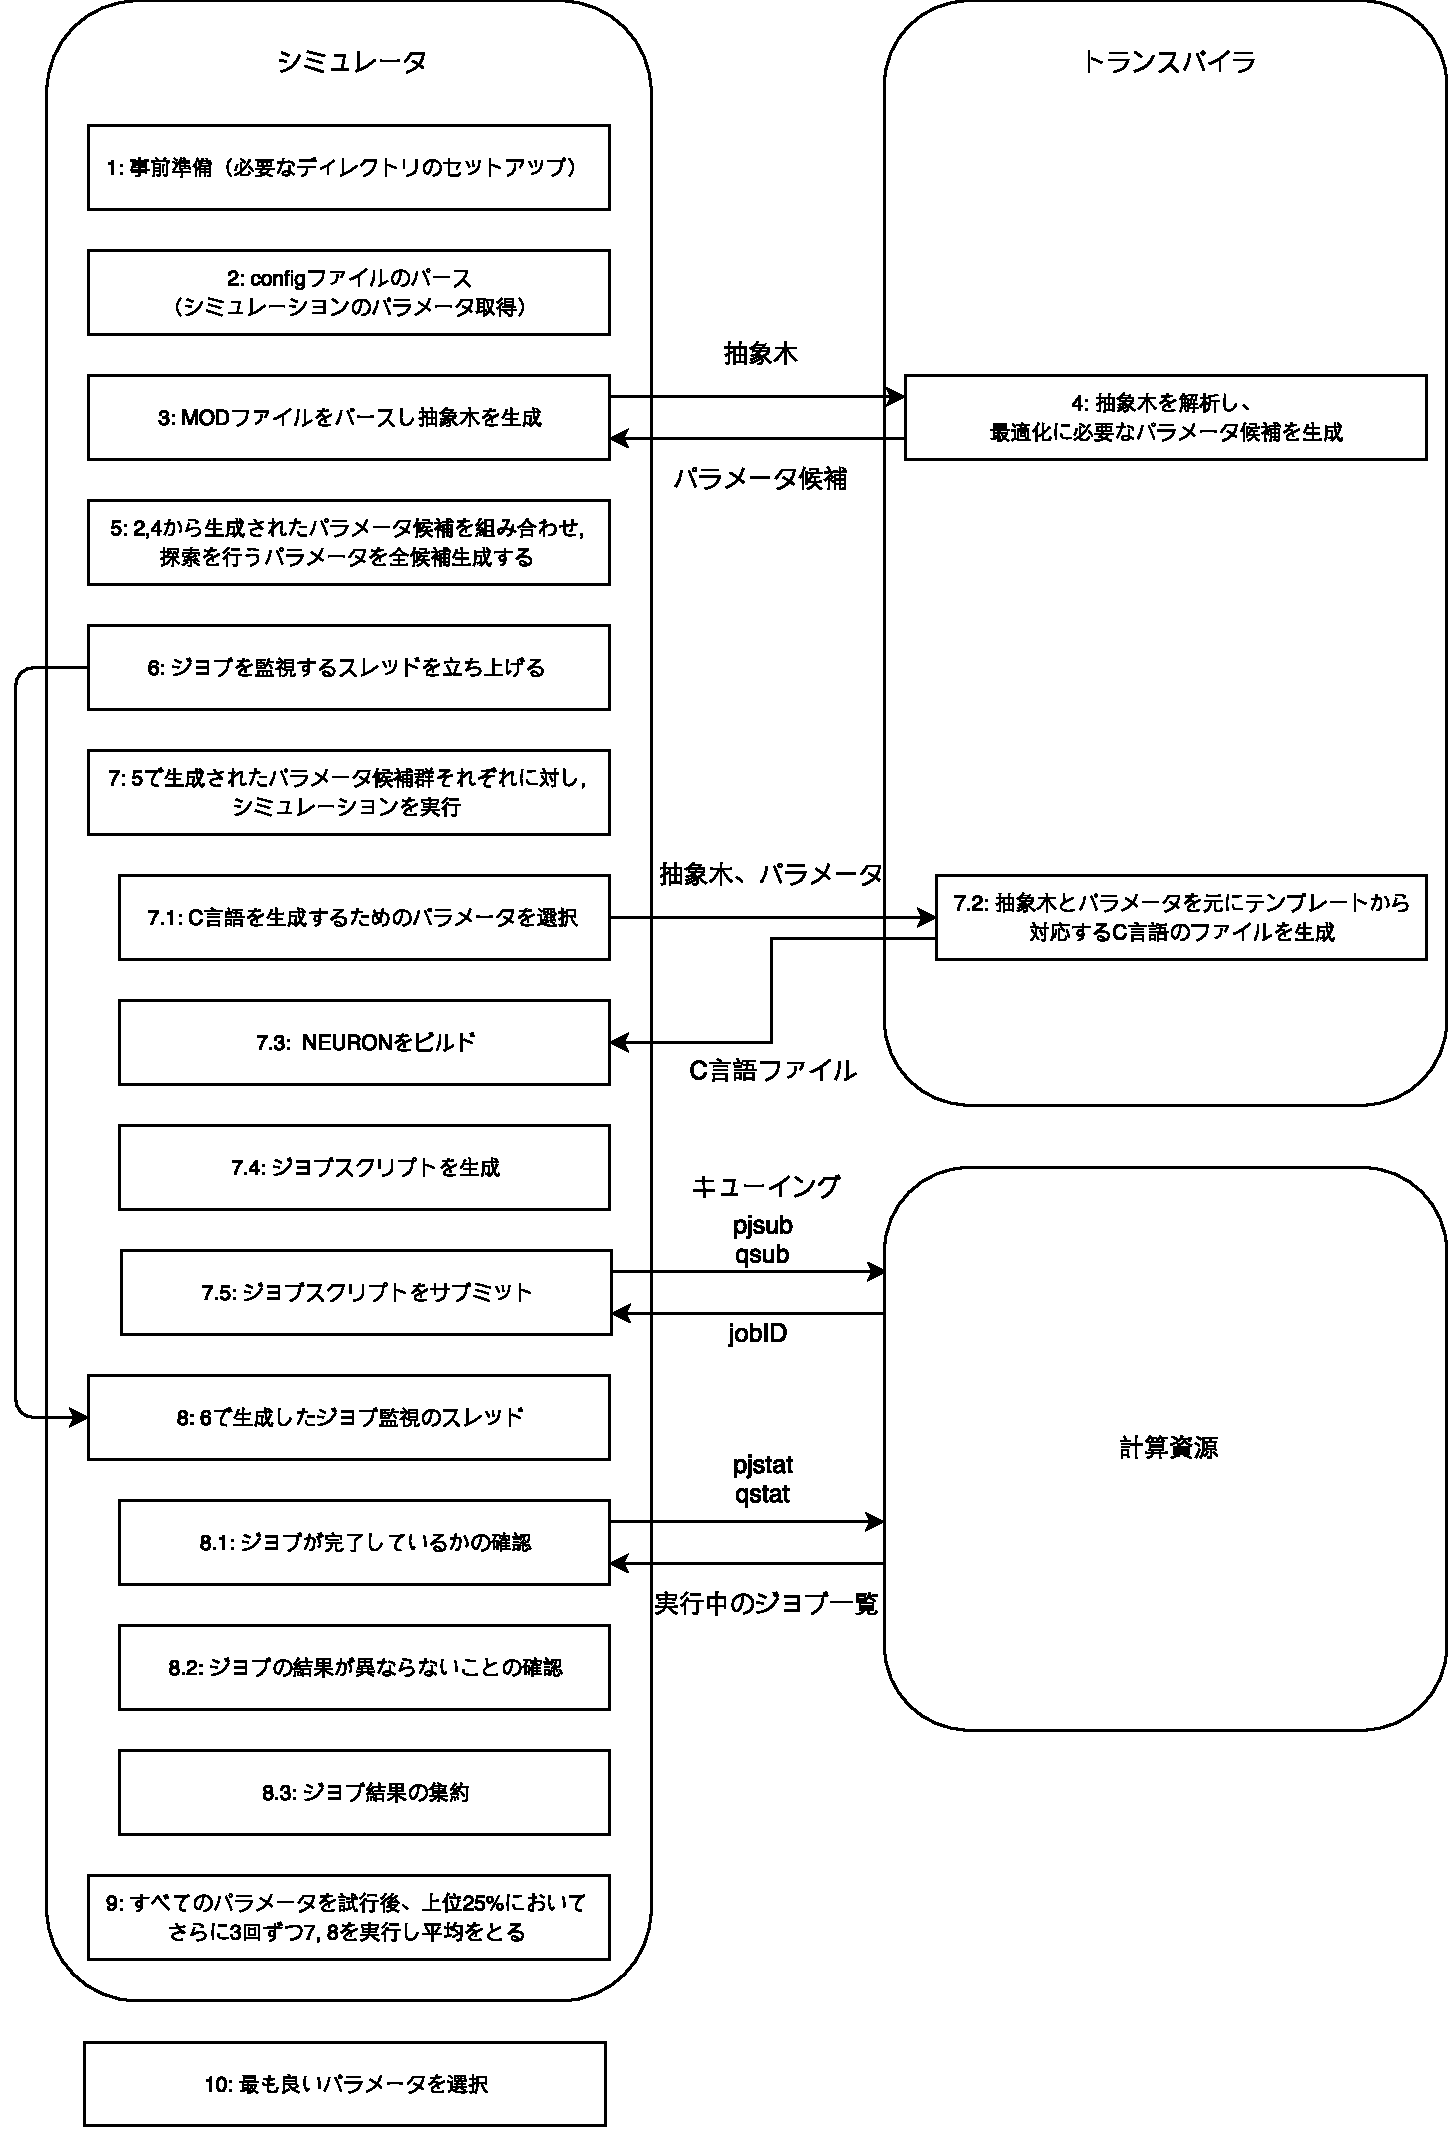
\includegraphics[width=1.1\textwidth]{./images/Genie.pdf}
    \caption{シミュレータの全体像}
    \label{fig:simulator-image}
 \end{center}
\end{figure}~\\

\clearpage

\subsubsection{事前準備}
シミュレータを起動した際, ジョブスクリプトやビルドスクリプトを置くためのディレクトリの作成や
並列でNEURONのビルドを行う場合に実行形式に対するレファレンスが衝突しないようにするため,
一時的に必要なディレクトリのコピーを作成するといったシミュレーションを行うために必要な
準備をはじめに行う.\\
 具体的には次に示すディレクトリを作成・初期化する.\\
\begin{table}[htb]
  \caption {作成されるディレクトリ}
{\footnotesize
\begin{framed}
\begin{verbatim}
  genie/ : rootディレクトリ
    |-- tmp/ : 実行結果, ログを保持するためのディレクトリ
    |-- neuron_kplus/
          |-- exec/ : 実行形式を保持するためのディレクトリ
          |-- exec.tmp/ : 並行ビルドのための exec のコピーディレクトリ
          |-- nrn-7.2.tmp/ : 並行ビルドのための nrn-7.2 のコピーディレクトリ
          |-- specials.tmp/ : 並行ビルドのための specials のコピーディレクトリ
\end{verbatim}
\end{framed}
}
\end{table}~\\

 この中で, 末尾に.tmpがつくディレクトリは並行してキューイングシステムにジョブをサブミットする際に
レファレンスが衝突しないようにするために必要となる.\\
 NEURONのシミュレーションはキューシステムにサブミットされたのち,順番が来るまでキューで待機状態にある. そして実行される段階になって初めてジョブスクリプトに指定されたNEURONの実行形式が参照される.\\
ここで実行形式を変更する必要がある際には,そこまでのジョブが完了してから再度ビルドから行うという方法を用いることもできるが,
その場合ビルドをする必要がある度にその間ジョブの実行を止めることになり,シミュレーション全体として大きなボトルネックになる.\\
 そこで, ビルドに関わるnrn-7.2, exec, specialsそれぞれのコピーとなる一時ディレクトリを作成し,ジョブスクリプトの内部から参照する
実行形式をビルドが必要な度に切り替えるようシミュレータ内部で設定することでレファレンスの衝突を起こさずにジョブを実行中に次に使う実行形式の
ビルドを行うことができるようになる.\\

\subsubsection{configファイルのパース}
\label{sec:simulator-config-parse}
シミュレーションを行う上で,どのシミュレーションファイルを用いるのか,パラメータとして何を利用するのか
といったシミュレーション自体の定義が必要となる. 本研究ではJSON形式で記述されたconfigファイルをシミュレータに渡すことで定義されたパラメータの範囲で
対象となるシミュレーションを最適化するためにパラメータの探索を行う.\\
 次にconfigファイルの例とともに,どのようにしてパラメータの範囲を定義するのかを示す.\\
configファイルでは, 実行形式の生成に関わるパラメータ(コンパイルオプションなど)とジョブスクリプトの生成に関わるパラメータを
分けて定義している. また, それぞれの環境に対して特有のパラメータについてはbuild\_config\_マシン名やjob\_マシン名というように,
末尾に実行マシンの名前をつけることで区別している.\\
\begin{table}[htb]
  \begin{center}
  \title{クラスタに対するconfigファイル}
{\footnotesize
\begin{lstlisting}[frame=single]
{
    # 実行形式の生成に関わるパラメータ
    "build" : {
        # ビルド対象のパスを定義
        "build": {
            "neuron_path": "../nrn-7.2",
            "specials_path": "../specials"
        },
        # クラスタのコンパイルオプションを定義
        "build_config_cluster": {
            "options": [
              "--without-iv",
              "--without-x",
              "--without-nrnoc-x11",
              "--with-paranrn",
              "--with-mpi",
              "--with-multisend",
              "--enable-shared=no",
              "--enable-static=yes"
            ],
            "compile_options": {
              "linux_nrnmech":"no",
              "use_pthread":"no",
              "CFLAGS":"\"-O3 -fopenmp -DKPLUS -DKPLUS_GATHER_SCATTER -DKPLUS_SPAWN -DCLUSTER_USE_OMP\"",
              "CXXFLAGS":"\"-O3 -fopenmp -DKPLUS -DKPLUS_GATHER_SCATTER -DKPLUS_SPAWN -DCLUSTER_USE_OMP\"",
              # 利用するコンパイラを定義する
              "CC":"mpicc, mpiicc"
            }
        }
    },
    # ジョブスクリプトの生成に関わるパラメータ
    "job" : {
        # クラスタのジョブスクリプトに関わるパラメータを定義
        "job_cluster": {
            # ノード数
            "nodes":"1",
            # MPIプロセス数
            "ppn":"2, 28, 2",
            # ロードするモジュールがある場合は定義
            "modules": [
            ],
            # OpenMPのスレッド数
            "omp_num_threads": "2, 16, 2",
            # 実行するコマンドを定義
            "nrniv": "../specials/x86_64/special -mpi",
            # 実行するシミュレーションを定義
            "hoc_name": "../hoc/bench_main.hoc",
            # シミュレーションのステップ数を定義
            "stop_time": 50,
            # NEURON本体でのループの分割数を定義
            "nthread": 16,
            # プロファイラを利用する場合はここで定義
            "prof": ""
        }
    }
}
\end{lstlisting}
}
\end{center}
\end{table}
\clearpage
configファイル内でパラメータの範囲を定義する際, 数字の場合はカンマで区切って範囲を定義する.
例としてOpenMPのスレッド数を指定する場合を考えると, 定義方法は3種類ありそれぞれ次に示すように解釈される.\\
\begin{table}[htb]
  \begin{center}
    \title{数値パラメータの定義}
{\footnotesize
\begin{framed}
\begin{verbatim}
# OpenMPのスレッド数
# パラメータ: "start, end"
"omp_num_threads": "2, 8"
# => [2, 3, 4, 5, 6, 7, 8]

# パラメータ: "start, end, step"
"omp_num_threads": "2, 8, 2"
# => [2, 4, 6, 8]

# パラメータ: "[parameters]"
"omp_num_threads": "[2, 4, 16]"
# => [2, 4, 16]
\end{verbatim}
\end{framed}
}
\end{center}
\end{table}~\\

文字列の候補を複数定義する場合は,
候補を\"[\", \"]\"でくくることでその中でカンマで区切られた文字列すべてを候補とすることができる.
\begin{table}[htb]
  \begin{center}
  \title {文字列パラメータの定義}
{\footnotesize
\begin{framed}
\begin{verbatim}
# 利用するコンパイラを定義する
"CC":"[mpicc, mpiicc]"
\end{verbatim}
\end{framed}
}
\end{center}
\end{table}~\\

\subsubsection{MODファイルをパースし抽象木を生成する}
\label{sec:simulator-mod-parse}
MODファイルのパースし抽象木を生成するにあたり, PythonのライブラリであるtextX\cite{textX-repo}を利用した. textXはパーサーとメタモデルを定義することで, 独自のDomain Specific Languagesを作成することができるという
Pythonのライブラリである.
その中でメタモデルについては, NEURONのMODファイルからNeuroMLという別の神経回路シミュレーションソフトの形式に変換する
ためのライブラリであるpynmodl\cite{pynmodl-repo}において作成されていたため, pynmodlのメタモデルを利用した.\\
 当初pynmodlを利用し, NeuroMLというXML形式の情報を利用し実装を行う予定だったが,
pynmodlはNeuroMLを開発しているチームの中で本論文を執筆時において開発中のライブラリであり
MODファイルから抽象木を取り出すためのメタモデルのみ実装されている段階であったため,
MODファイルからtextX形式の抽象木を生成するプログラムとして利用した.\\

\subsubsection{パラメータ候補群の生成}
\ref{sec:simulator-config-parse}項と\ref{sec:simulator-mod-parse}項で生成したパラメータ群がシミュレータで探索する対象となる.\\
パラメータは大きく,
\begin{enumerate}
\item Configファイルに定義されるNEURON本体のコンパイルに関わるパラメータ(コンパイルオプション)
\item Configファイルに定義されるジョブスクリプト生成に関わるパラメータ(MPIプロセス数やOMPスレッド数など)
\item MODファイルから抽出されたC言語の生成に関わるパラメータ
\end{enumerate}
に分けられ, 本論文執筆時においてはこれらのパラメータのすべての組み合わせを候補群として生成し最適化を図る.\\
 また,パラメータ候補群を生成するループの順番を実行形式に関わるコンパイルオプションとC言語の生成に関わるパラメータを外側に,
ジョブスクリプトの生成に関わるパラメータを内側にすることで, ジョブの完了を待っている間に必要がある場合は次の実行形式をビルドする
ことができる.\\
{\footnotesize
\begin{lstlisting}[title=パラメータ候補の生成 疑似コード,frame=single]
# 未実行のシミュレーションのパラメータを保持する配列
pending_sims = []

# それぞれのパラメータに対して3重のループを組み, 全通りのパラメータ候補群を生成
for compile_param in compile_params {
    for code_optimize_param in code_optimize_params {
        for job_param in job_params {
            pending_sims.append([compile_param, code_optimize_param, job_param])
        }
    }
}
\end{lstlisting}
}

\subsubsection{パラメータ候補群に対してシミュレーションを実行}
シミュレーションの実行は,
\begin{enumerate}
\item ジョブ実行スレッドを生成するループ
\item ビルドが必要となるかの判定やパラメータの記録を行うジョブのサブミットの前後処理をする関数.
\item ビルドとジョブのサブミットを行う関数.
\end{enumerate}
という3工程で行われる.

\paragraph{ジョブ実行スレッド生成ループ}~\\
 このループでは, 未実行のシミュレーションを保持している配列が空になるまで
ジョブ実行のためのスレッドを逐次生成していく.\\
 その際, 連続して多数のジョブを投げることで他のシステム利用者に迷惑をかけることがないよう,
事前に設定したジョブの最大同時実行数を超えないようにする必要がある.
実装においては, 外側のループを未実行のシミュレーションが存在する限り続け,
実行中のジョブの数が最大同時実行数を超える場合は一定時間スリープを行うという形にした.\\
 また, ジョブのサブミットを別スレッドで行うため, ジョブの実行順が変わると本来必要のないビルドが必要となる場合があることから
スレッドを生成したのちにわずかな時間スリープさせることにした.\\

{\footnotesize
\begin{lstlisting}[title=ジョブ実行スレッドを生成するループ 疑似コード,frame=single]
MAX_NUM_JOBS = 4
run() {
    # キューイングシステムのジョブ実行状況を監視するメソッドを別スレッドで生成
    thread.start(watch_job)
    current_sim_num = 0
    # 未実行のシミュレーションが存在する場合はループを続ける
    while pending_sims.size() != 0 {
        # 現在実行中のジョブの数が最大同時実行数を超えている場合は待機する
        if current_sim_num > MAX_NUM_JOBS {
            sleep(15)
        }
        # 実行中のジョブの数が最大同時実行数になるまでジョブをサブミットする
        while True {
            if current_sim_num >= MAX_NUM_JOBS {
                break
            }
            # ジョブのサブミットを別スレッドで行う
            thread.start(deploy_job)
            current_sim_num += 1
            # ジョブのサブミットを別スレッドで行うため,スレッドの生成を少しずらす
            time.sleep(1)
        }
    }
}
\end{lstlisting}
}

\paragraph{ジョブサブミットの前後処理}~\\
 ジョブのサブミットは並行して生成されたスレッド上で行われる. そのためその前処理として
mutexロックをかけた上で, 今回利用するパラメータの取得(pending\_simsから先頭の要素を取り出す)や
ビルドが必要か否かを判断する際に使う最新のパラメータの更新といった処理が必要となる.\\
 後述するジョブのサブミットを行う関数を呼ぶことでジョブIDを取得することができるが, そのジョブIDに関連した処理が後処理となる.\\
一つは, ジョブの監視に利用する実行中のジョブIDを保持したテーブルに取得したジョブIDを追加することで,
もう一つはジョブIDと紐付けてパラメータを結果を保存するテーブルに追加することである. こうしてジョブIDとパラメータを紐付けることで, そのジョブが完了した際にジョブIDを通して実行時間とパラメータを関連づけることができるようになる.\\

{\footnotesize
\begin{lstlisting}[title=ジョブサブミットの前後処理 疑似コード,frame=single]
# 実行中のジョブの状態を保持したテーブルでジョブの完了を判断するために利用する
# running_jobs[job_id] が 0 の場合は, job_id が pjstat や qstat の出力に一度も現れていない状態
# 1 の場合は, job_id が pjstat や qstat の出力に一度は現れている状態
running_jobs = {}

deploy_job() {
  if pending_sims.size() > 0:
      # 未実行のシミュレーションのパラメータを一つ取り出す
      compile_param, code_optimize_param, job_param = pending_sims.pop(0)

      # 実行形式生成に関わるパラメータが直前に利用したパラメータと異なる場合は
      # 実行形式をビルドし直す必要がある
      shouldBuild = current_compile_param != compile_param or
                    current_code_optimize_param !0 code_optimize_param

      # サブミットするジョブに用いたパラメータをもっとも直近のものとして更新する
      current_compile_param = compile_param
      current_code_optimize_param = code_optimize_param

      # パラメータを元に実効形式, ジョブスクリプトを生成しジョブをサブミットする
      # 返り値は jobID となる
      job_id = deploy(shouldBuild,
                      compile_param,
                      code_optimize_param,
                      job_param)

      # job_id を完了判定のためのテーブルに初期状態として記録する
      running_jobs[job_id] = 0

      # 今回のシミュレーションで利用したパラメータと jobID を結果を保持するテーブルに保存するためまとめる
      merge_params = compile_param +
                     code_optimize_param +
                     job_param +
                     {"job_id": job_id, "time": 0}
      # パラメータと実行結果を保存するテーブルにパラメータを追加
      # ジョブが完了した段階で jobID を元に time を更新する
      result_table.add(merge_params)
}

\end{lstlisting}
}
\paragraph{ジョブのサブミット}~\\
 ジョブのサブミットを行う関数では, 実行形式の生成とジョブスクリプトの生成そしてキューイングシステムに対してジョブをサブミットするという3つの役割を持つ.\\
 まずはじめに, 実行形式の生成を行う必要があるのは実行形式の生成に関与するパラメータが現在利用されている実行形式のものと異なる場合であるが,
それはcompile\_paramとcode\_optimize\_paramを比較してやればよく, その結果がshouldBuildに入っているためこの変数を利用することで判定できる.\\
 実行形式を改めて生成しなおす必要がある場合, すでにサブミットされたジョブスクリプトから参照されている可能性のある実行形式を変更するとシミュレーション結果が異なる可能性が高いので
ディレクトリを切り替えることで参照の衝突を防ぐ必要がある. ここでは, use\_tmpと言う変数を用いて現在の実行形式は一時ディレクトリに存在するものか
オリジナルのディレクトリに存在するものかの判別を行っており, 仮にuse\_tmpの値が真である場合は元のディレクトリ名の末尾に .tmp がついたディレクトリを利用することになる.\\

また, ジョブスクリプトを生成するにあたり, そのファイル名を各ジョブごとに一意にする必要がある.\\
 これは実行形式の場合と同様にキューイングシステムで順番が回ってきた時にジョブスクリプトが参照されるため,
サブミットされた後に順番が回ってくる前にジョブスクリプトが更新されると本来関係のないパラメータを用いてシミュレーションすることになるからである.\\
 本研究ではジョブの数を保持しておき, ジョブスクリプトを job + "何番目のジョブか" + .shという形(job1.sh, job2.sh, ...)で生成することで参照の衝突を防いだ.\\

実行形式のビルド, ジョブのサブミットに関してはコマンドが決まっているためShell Scriptをあらかじめ用意しておき,
そのShell Scriptに引数として一時ディレクトリを使用するか否か, 何番目のジョブかといった情報を与えることで行った.\\

{\footnotesize
\begin{lstlisting}[title=ジョブのサブミット 疑似コード, frame=single]

deploy(shouldBuild, compile_param, code_optimize_param, job_param) {
    # 一時ディレクトリを利用するかという情報を退避する
    _use_tmp = use_tmp

    # 実行形式を再度生成する必要がある場合
    if shouldBuild {
        # 現在利用しているディレクトリは使えないため, ディレクトリのフラグを切り替える
        use_tmp = not use_tmp

        # 始めの行で退避していた情報を更新する
        _use_tmp = use_tmp

        # C言語のファイルをMODファイルの情報を元に生成する
        transpiler.gen(code_optimize_param)

        # コンパイルに関わるパラメータと実行形式を生成するディレクトリの情報を用いて
        # NEURONの実行形式を生成する
        build(compile_param, _use_tmp)
    } else {
        # ジョブスクリプトへのリファレンスの衝突を防ぐため,何番目のジョブかという情報を保持する
        job_cnt += 1

        # ジョブスクリプトに関わるパラメータとどのディレクトリの実行形式を利用するのかと言う情報を元に,
        # ジョブスクリプトを "job" + job_cnt + ".sh"と言うフォーマットで生成し(job1.sh, job2.sh, ... ),
        # キューイングシステムにサブミットする
        job_id = submit(job_params,
                        job_cnt,
                        _use_tmp)
        return job_id
    }
}
\end{lstlisting}
}

尚, ビルドスクリプトに対して与える引数は次の3つになる.\\
\begin{enumerate}
\item 実行マシンに依存する命令セット名(クラスタではx86\_64, 京ではsparc64)
\item 最適化したC言語のファイルを使うか否か(Pythonから呼び出され, パラメータはbooleanなので文字列比較を行っている)
\item 実行形式を生成するパス(一時ディレクトリを用いるかオリジナルのディレクトリを用いるかを決定するため, ".tmp"または""が与えられる)
\end{enumerate}
{\footnotesize
\begin{lstlisting}[title=実行形式のビルドスクリプト, frame=single]
#!/bin/bash -x

ARCH=$1

rm -r ${ARCH}
../exec$2/${ARCH}/bin/nrnivmodl ../mod
if [ $# -eq 1 ]
then
    echo "optimized"
    rm ./${ARCH}/hh_k.c
    cp ~/genie/genie/transpiler/tmp/hh_k.c ${ARCH}/hh_k.c
else
    if [ $2 == 'True' ]
        echo "optimized"
        rm ./${ARCH}/hh_k.c
        cp ~/genie/genie/transpiler/tmp/hh_k.c ${ARCH}/hh_k.c
    then
        echo "default"
    else
    fi
fi
../exec$2/${ARCH}/bin/nrnivmodl ../mod
\end{lstlisting}
}

ジョブのサブミットに際しては, ジョブの番号を与えることで一意にジョブスクリプトを指定することができるため,
ジョブの番号を引数として与える.\\
{\footnotesize
\begin{lstlisting}[title=ジョブのサブミットスクリプト, frame=single]
#!/bin/bash -x
qsub ../../genie/simulator/tmp/job$1.sh
\end{lstlisting}
}

\subsubsection{ジョブ実行の監視}
ジョブ実行の監視は,
\begin{enumerate}
\item ジョブ実行の監視とジョブ実行の後処理(パラメータと実行時間の関連付け)を行う関数
\item 実行中のジョブの完了判定
\item ジョブの結果を集約する関数
\item ジョブの結果が一致していることを確認する関数.
\end{enumerate}
の4つから構成される.\\
\paragraph{ジョブ実行の監視と後処理}~\\

ジョブの実行スレッドを生成するループの頭で実行中のジョブの監視スレッドは立ち上げられ,
以降ジョブの実行とは関係なく定期的に繰り返し実行される.\\
 一度の実行では, キューイングシステムに対してqstatやpjstatを利用して実行中のジョブの情報を取得し,
現在実行中のジョブIDそれぞれを比較する. ここでもしジョブが完了している場合は,
ジョブ結果の集約を行い, ジョブIDを元に結果をテーブルに書き込みそして実行中のテーブルからジョブIDを削除する.\\
 ジョブ完了時にすでに実行中のジョブの数が最大同時実行数に達していた場合は, ここでcurrent\_job\_numの値が1つ減ることで
次のループで新たにジョブをサブミットできるようになる.\\

また, 未実行のシミュレーションがなくなり, 現在実行中のジョブがすべて完了した段階でパラメータ候補すべてに対してシミュレーションをし終えたといえるため
ジョブ結果が最適化を通して変わっていないかの確認とパラメータと実行時間を保持したテーブルのCSV形式での書き出しを行いシミュレータを終了する.\\
{\footnotesize
\begin{lstlisting}[title=ジョブ実行の監視と後処理 疑似コード, frame=single]
watch_job() {
    # 実行中のジョブすべてに対して, ジョブが完了しているかの確認を行う
    for job_id in running_jobs {
        # ジョブが完了している場合, ジョブ結果の集約を行う
        if not is_job_still_running(job_id) {
            # jobID に紐付いたジョブ結果の集約(実行にかかった時間の取得)
            time = summary(job_id)

            # 結果を保持するテーブルの jobID に紐付いた実行時間を更新する
            result_table['job_id' == job_id]['time'] = time

            # 現在実行中のジョブから jobID を削除する
            running_jobs.remove(job_id)
            current_job_num -= 1
        }
    }

    # 未実行のシミュレーションと現在実行中のジョブが一つもない時,
    # すべてのシミュレーションが終わったと見なせるので, 実行結果が異ならないかの確認を行う
    if len(pending_sims) == 0 and len(running_jobs) == 0 {
        # 実効結果が最適化によって異ならないかの確認を行う
        if verify() {
            print("All results are the same.")
        } else {
            print("Some results are different.")
        }
        # 実効結果とパラメータを保持したテーブルを CSV 形式で保存する
        result_table.to_csv("result.csv")
        return
    }
    # シミュレーションがすべて終わっていない時は,ジョブの監視スレッドを再度立ち上げ直す
    sleep(5)
    thread.start(watch_job)
\end{lstlisting}
}

\paragraph{ジョブの完了判定}~\\
 ジョブの完了判定を行う際には, キューイングシステムの上でのジョブの実行状況を取得するpjstatとqstatの出力結果を利用する.\\
 これらの出力結果が常に一定のフォーマットに従うことは\ref{subsec:job-env}項で示したが, 一定の出力を持つため正規表現を用いることでジョブIDとその実行状況を取得可能である.
ここで注意することは, ジョブの監視スレッドの実行が一定間隔であり,
必ずしもqstatやpjstat実行時にCやSTOといったジョブが完了した状態であるという出力が得られるとは限らないことである.\\
 一方で, ジョブがキューイングシステム内で待機状態や実行状態である時間はジョブの監視スレッドの実行間隔より十分に大きいため,
キューイングシステム内に特定のジョブIDに紐づくジョブが存在しているという記録を残すことは容易である.\\
 以上からジョブの完了の判定は, ジョブが完了状態であるという情報をキューイングシステムから得ることができればその情報を利用し,
取得できなかった場合はキューイングシステム上にジョブが存在しなくなった段階でそのジョブは完了しているとみなすことができる.\\

{\footnotesize
\begin{lstlisting}[title=ジョブ完了判定 疑似コード, frame=single]
# qstat の出力に対してジョブ ID とジョブの実行状況を取得するための正規表現
job_cluster_exp = re.compile(
    "(?P<id>\d+).\w+\s+\w+.\w+\s+\w+\s+\d+:\d+:\d+\s+(?P<state>\w+)\s+\w+\s+")

# pjstat の出力に対してジョブ ID とジョブの実行状況を取得するための正規表現
job_k_exp = re.compile(
    "(?P<id>\d+)\s+\w+.\w+\s+\w+\s+(?P<state>\w+)\s+[\s\w\d\[\]\/\:\-]+")

is_job_still_running(job_id) {
    # 京とクラスタでは用いるコマンドが違うため分岐する必要がある(qstatとpjstatの違い)
    if environment == "cluster" {
        # qstat コマンドを実行し実行中のジョブの状態を取得する
        res = execute("qstat")

        # 改行(\n)で連結された一つの文字列となっているため, 行ごとに分離する
        job_lines = res.split('\n')

        # コマンドの結果の行に対してそれぞれ正規表現と一致するか確認をする
        # ジョブ ID が存在しない場合は, まだキューイングシステムにサブミットされていないか, すでに完了してキューイングシステムからの出力に表示されていないという2つのパターンが考えられるため,running_jobs にジョブの状態を保持することで判断する
        for line in job_lines {
            m = job_cluster_exp.match(line)

            # 一致する場合, ジョブの実行状況を記録する
            if m is not None {
                state = m.group("state")
                # ジョブ ID がその行と一致し, かつジョブの状態がC(Complete)であるならば, ジョブは完了したと見なせる
                if job_id == m.group("id") {
                    if state == "C" {
                        return False
                    } else {
                        # ジョブがまだ完了していないため, ジョブ ID に紐付いたジョブがキューイングシステムにサブミットされた状態であると記録する
                        if running_jobs[job_id] == 0 {
                            running_jobs[job_id] = 1
                            return True
                        }
                    }
                }
            }
        }
        # ここまでで関数の実行が終わっていないのは qstat の出力にジョブ ID が含まれていないということである. その上で, 一度でもキューイングシステムの出力に現れているのであればジョブは完了しているとみなし,そうでないならばまだサブミットされていないとみなす
        if running_jobs[job_id] > 0 {
            return False
        } else {
            return True
        }
    } else if environment == "k" {
        res = execute("pjstat")
        job_lines = res.split('\n')
        for line in job_lines {
            m = job_k_exp.match(line)
            if m is not None {
                state = m.group("state")
                if job_id == m.group("id") {
                    if running_jobs[job_id] == 0 {
                        running_jobs[job_id] = 1
                        return True
                    }
                }
            }
        }
        if running_jobs[job_id] > 0 {
            return False
        } else {
            return True
        }
    }
}
\end{lstlisting}
}

\paragraph{ジョブ結果の集約}~\\
 ジョブ結果は job + ジョブの順番 + .sh.o + ジョブIDという形(job1.sh.o10000, job2.sh.o10001)で出力される.
また, 結果として出力される内容の中で実行時間を出力している行は複数のプロセスやスレッドで並行的に計算をしているため順番は前後するものの
同一のフォーマットに従うため, すべての行の中からこのフォーマットに合致する行を探すことで実行時間を取得することができる.\\
{\footnotesize
\begin{lstlisting}[title=ジョブ結果の集約 疑似コード, frame=single]
# シミュレーション結果のファイルの中で実行時間を取得するための正規表現
time_exp = re.compile(
    "\s+\* core time : (?P<decimal>\d+).(?P<float>\d+) sec\s+")

summary(job_id, job_cnt) {
    # ジョブ ID とジョブの順番を元に, ジョブ結果のファイル名を作り実行時間を取得する
    core_time = obtain_time("job{0}.sh.o{1}".format(job_cnt, job_id))
    return core_time
}

obtain_time(filename) {
    # 与えられたファイル名のファイルに対するアクセスを作る
    f_check = Path("{0}".format(filename))

    # 与えられたファイル名のファイルがまだ存在していない場合待機をする
    while not f_check.exists() {
        time.sleep(5)
    }
    f = open("{0}{1}".format(dir_path, filename))
    lines = f.readlines()
    f.close()

    # ファイルの行全てに対して一行ずつ正規表現と一致する行があるか確認する
    for line in lines {
        m = time_exp.match(line)
        if m {
            # 正規表現で取得した整数部と小数部を実行時間に変換する
            calc_time = int(m.group("decimal")) +\
                        int(m.group("float")) * 10**(-len(m.group("float"))+1)
            return calc_time
        }
    }
}
\end{lstlisting}
}

\paragraph{ジョブ結果の比較}~\\
 最後に,実際の実行結果が最適化を通して変化していないことの確認も必要である.\\
 これは実行結果のファイルを見ることで判断できるが, 複数プロセス・スレッドを用いた場合途中の出力結果の順番がランダムになっているという問題があった.
この問題を解決するため, 実行結果に直接関わる部分のみを抜き出してソートし比較することで実行結果が同一であることを確認した.\\
まず, シミュレーション系においてジョブの実行結果は次に示される3つの関数で出力されていた.\\
{\footnotesize
\lstinputlisting[title=ジョブ実行結果出力箇所,label=job-output-setting,frame=single]{src/job/output-setting}
}
またその実行結果を一部抜粋した元が次になる.\\
{\footnotesize
\lstinputlisting[title=ジョブ実行結果一部抜粋,label=job-output,frame=single]{src/job/output}
}
仮に同じシミュレーションをシングルプロセス・シングルスレッドで行った場合,上記の結果は
{\footnotesize
\lstinputlisting[title=シングルスレッドで実行する場合の実行結果,label=job-output-sorted,frame=single]{src/job/output-sorted}
}
のようにIDが昇順になる.\\
 そのため,3種類の関数print\_stat, spikeout, printSpikeStatからの出力結果をそれぞれソートした上で比較することで実行結果が同一であることを確かめることができる.\\
 本研究においては, それぞれの関数で出力形式が一定であり, 上記の3種類の関数のみがシミュレーションの実行結果と関係しているため,
IDを元にそれぞれの出力結果を並べ替え, ソート後の出力結果を格納した配列のハッシュ値を比較することで実行結果に変化がないことを確かめた.\\
{\footnotesize
\lstinputlisting[title=実行結果比較コード,label=compare-job-output,frame=single]{src/python/compare-job-output.py}
}

\subsubsection{シミュレーションの再実行}
シミュレーションを各パラメータに対して一度だけ実行する場合, 並列でジョブを投入しているため
メモリ利用状況や他のプロセスの影響も含めて実行時間が状況に応じてある程度変化することが予測される.\\
 そのため,複数回試行した上でその平均実行時間がもっとも短いものを選択するという方法を取り,
外部からの影響を減らすことを試みた.\\
 しかしながらパラメータ候補群を全探索する方法で複数回のシミュレーションを行うには非常に時間がかかるため,
探索範囲を一度目のシミュレーション結果を元に絞り込むことで探索範囲を狭めることができると考え,
本研究においては初回シミュレーションの上位25\%を対象として複数回のシミュレーションを行う形をとることとした.\\
